% Chapter Template

\chapter{Ensayos y resultados} % Main chapter title
En este capítulo se detallan los ensayos realizados en las formaciones ferroviarias y en los talleres de Trenes Argentinos. El orden cronológico de los ensayos es distinto al del desarrollo del firmware. En este documento se ha presentado previamente el diseño de la solución para facilitar la comprensión del trabajo realizado. El desarrollo de la solución fue posterior a una serie de mediciones realizadas en los talleres que permitieron identificar parámetros clave del sistema. \\

En las secciones que siguen se explican las mediciones realizadas en las visitas a los talleres de Victoria y Castelar de Trenes Argentinos Operaciones. Luego se presenta un análisis de datos de las tramas relevadas y también las pruebas de integración propuestas para validar el desarrollo. \\


\label{Chapter4} % Change X to a consecutive number; for referencing this chapter elsewhere, use \ref{ChapterX}

%----------------------------------------------------------------------------------------
%	SECTION 1
%----------------------------------------------------------------------------------------
\section{Ensayos en trenes para medir datos de la red TCN y PIDS}
Uno de los objetivos generales del proyecto en el que se enmarcó este trabajo, era relevar las soluciones existentes de la red TCN y PIDS. A lo largo del desarrollo, se realizaron reuniones de trabajo con el personal de Trenes Argentinos Operaciones, y visitas a los talleres de la Gerencia de material rodante eléctrico para relevar información técnica. En orden cronológico, incluyendo trabajo realizado en etapa de confinamiento por COVID-19, se resaltan las siguientes interacciones con SOFSE:\\


\begin{enumerate}

\item 2020-05-20: se ensayaron mediciones sobre la maqueta de los talleres de Castelar, coordinadas de forma remota, para obtener mediciones de datos de la red RS485 del sistema PIDS.

\item 2020-06-30: se ensayaron mediciones sobre formaciones ferroviarias operativas en los talleres de Victoria, relevando los puntos de interconexión de la red TCN con el TLCD (pantalla táctil del conductor). Se realizaron también mediciones en el punto de interconexión del bus MVB con el módulo RCMe. 

\item 2020-09-23: se ensayaron nuevas mediciones, coordinadas de forma remota, en la maqueta de Castelar con un nuevo módulo analizador de datos.

\item 2021-04-09: se relevaron los puntos de interconexión entre RCMe y el PIDS, y entre los módulos IDU y SCU en formaciones operativas en los talleres de Victoria. También se ensayaron mediciones sobre el bus de datos RS485 que conecta el SCU con la DACU.

\item 2021-06-04: se ensambló una maqueta local usando un cartel led compatible con la serie de los carteles de trenes relevados y se presentó como informe de avance.

\item 2022-08-11, CASE 2022.

\end{enumerate}

Durante las visitas a los talleres de Victoria, se pudo acceder a los planos eléctricos del sistema de comunicaciones del tren. Esta información resultó muy relevante ya que permitió comprender la lógica de interconexión de los módulos del tren y preparar un sistema de medición. Como consecuencia de las visitas, se fueron desarrollando piezas sueltas de hardware para realizar mediciones in-situ, a partir del relevamiento de los conectores y conexiones entre módulos.\\

\section{Arreglo experimental para realizar mediciones}

Las redes del sistema PIDS y TCN siguen el estándar RS-485. Este tipo de redes es muy utilizada para transmisión y recepción de datos, ya que tiene interfaces eléctricas muy robustas que usan señales diferenciales, y que normalmente se implementan en cables de par trenzado, permitiendo cableados largos con buena inmunidad al ruido eléctrico. \\
 


\begin{figure}[ht]
	\centering
	%\includepdf[pages={1}, angle=90]{./Figures/output.driverled.pdf}
	\includegraphics[width=1.66\textwidth, angle=90]{./Figures/setupMediciones.png}
	\caption{.}
	\label{fig:setupMediciones}
\end{figure}

\section{Análisis de datos experimentales}


\section{Pruebas sobre maqueta en talleres ferroviarios}


En el circuito esquemático de la figura \ref{fig:schDriverled} se presenta el detalle de conexiones eléctricas entre bloques. Se puede observar que a la salida del conector de datos (CONN 2x8) hay dos buffers de la serie 74HC245D que direccionan las señales eléctricas a izquierda y derecha del arreglo de matrices led. A izquierda viajan las señales SER(data), SRCLK (Clock) y XXX (latch) al arreglo de Shift Registers de la serie 74HC595. Por la derecha se maneja la habilitación secuencial de las filas a través de un arreglo de decodificadores 3x8 de la serie 74HC138. Cada salida de los decodificadores se conecta a un driver de corriente en arreglo de transistores MOSFET FDS4953. Estos decodificadores cableados adecuadamente permiten manejar las 32 señales de un cartel de 4x8 módulos led. \\


\begin{figure}[ht]
	\centering
	%\includepdf[pages={1}, angle=90]{./Figures/output.driverled.pdf}
	\includegraphics[width=1.66\textwidth, angle=90]{./Figures/output.driverled.pdf}
	\caption{Circuito esquemático de la placa controladora de los carteles de matriz led.}
	\label{fig:schDriverled}
\end{figure}


\begin{figure}[ht]
	\centering
	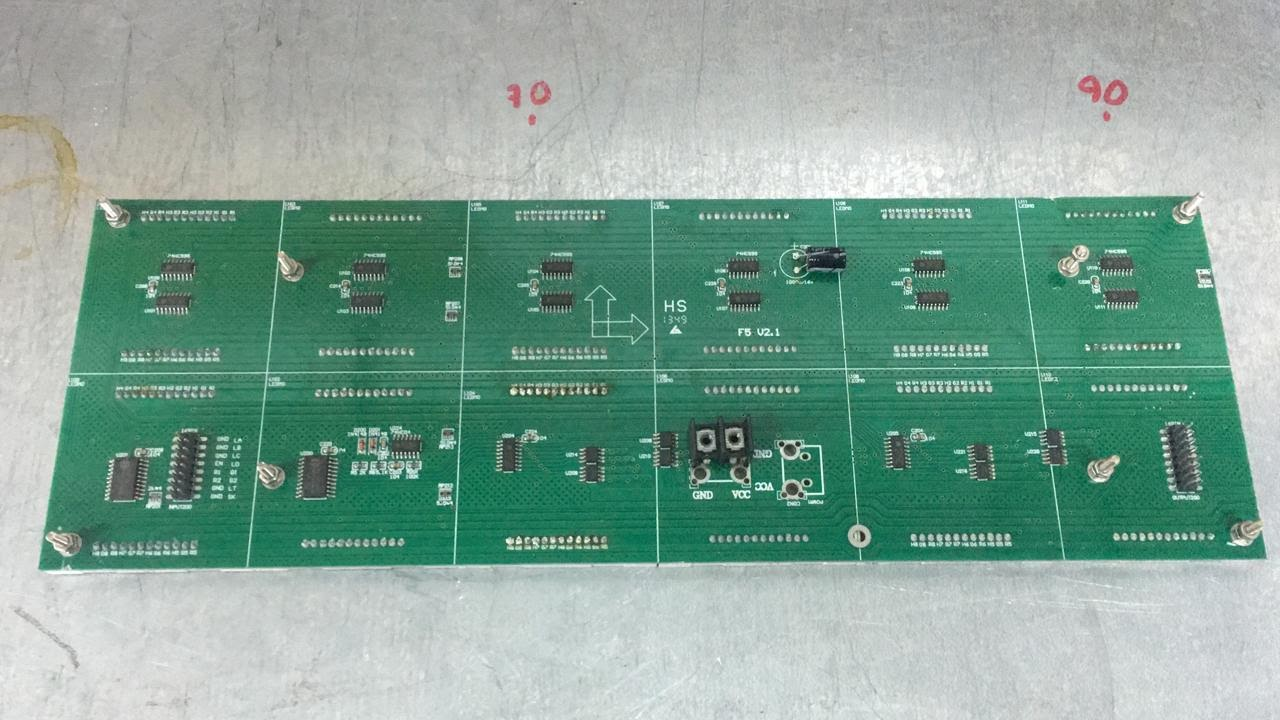
\includegraphics[width=1\textwidth]{./Figures/cartel2x6.jpeg}
	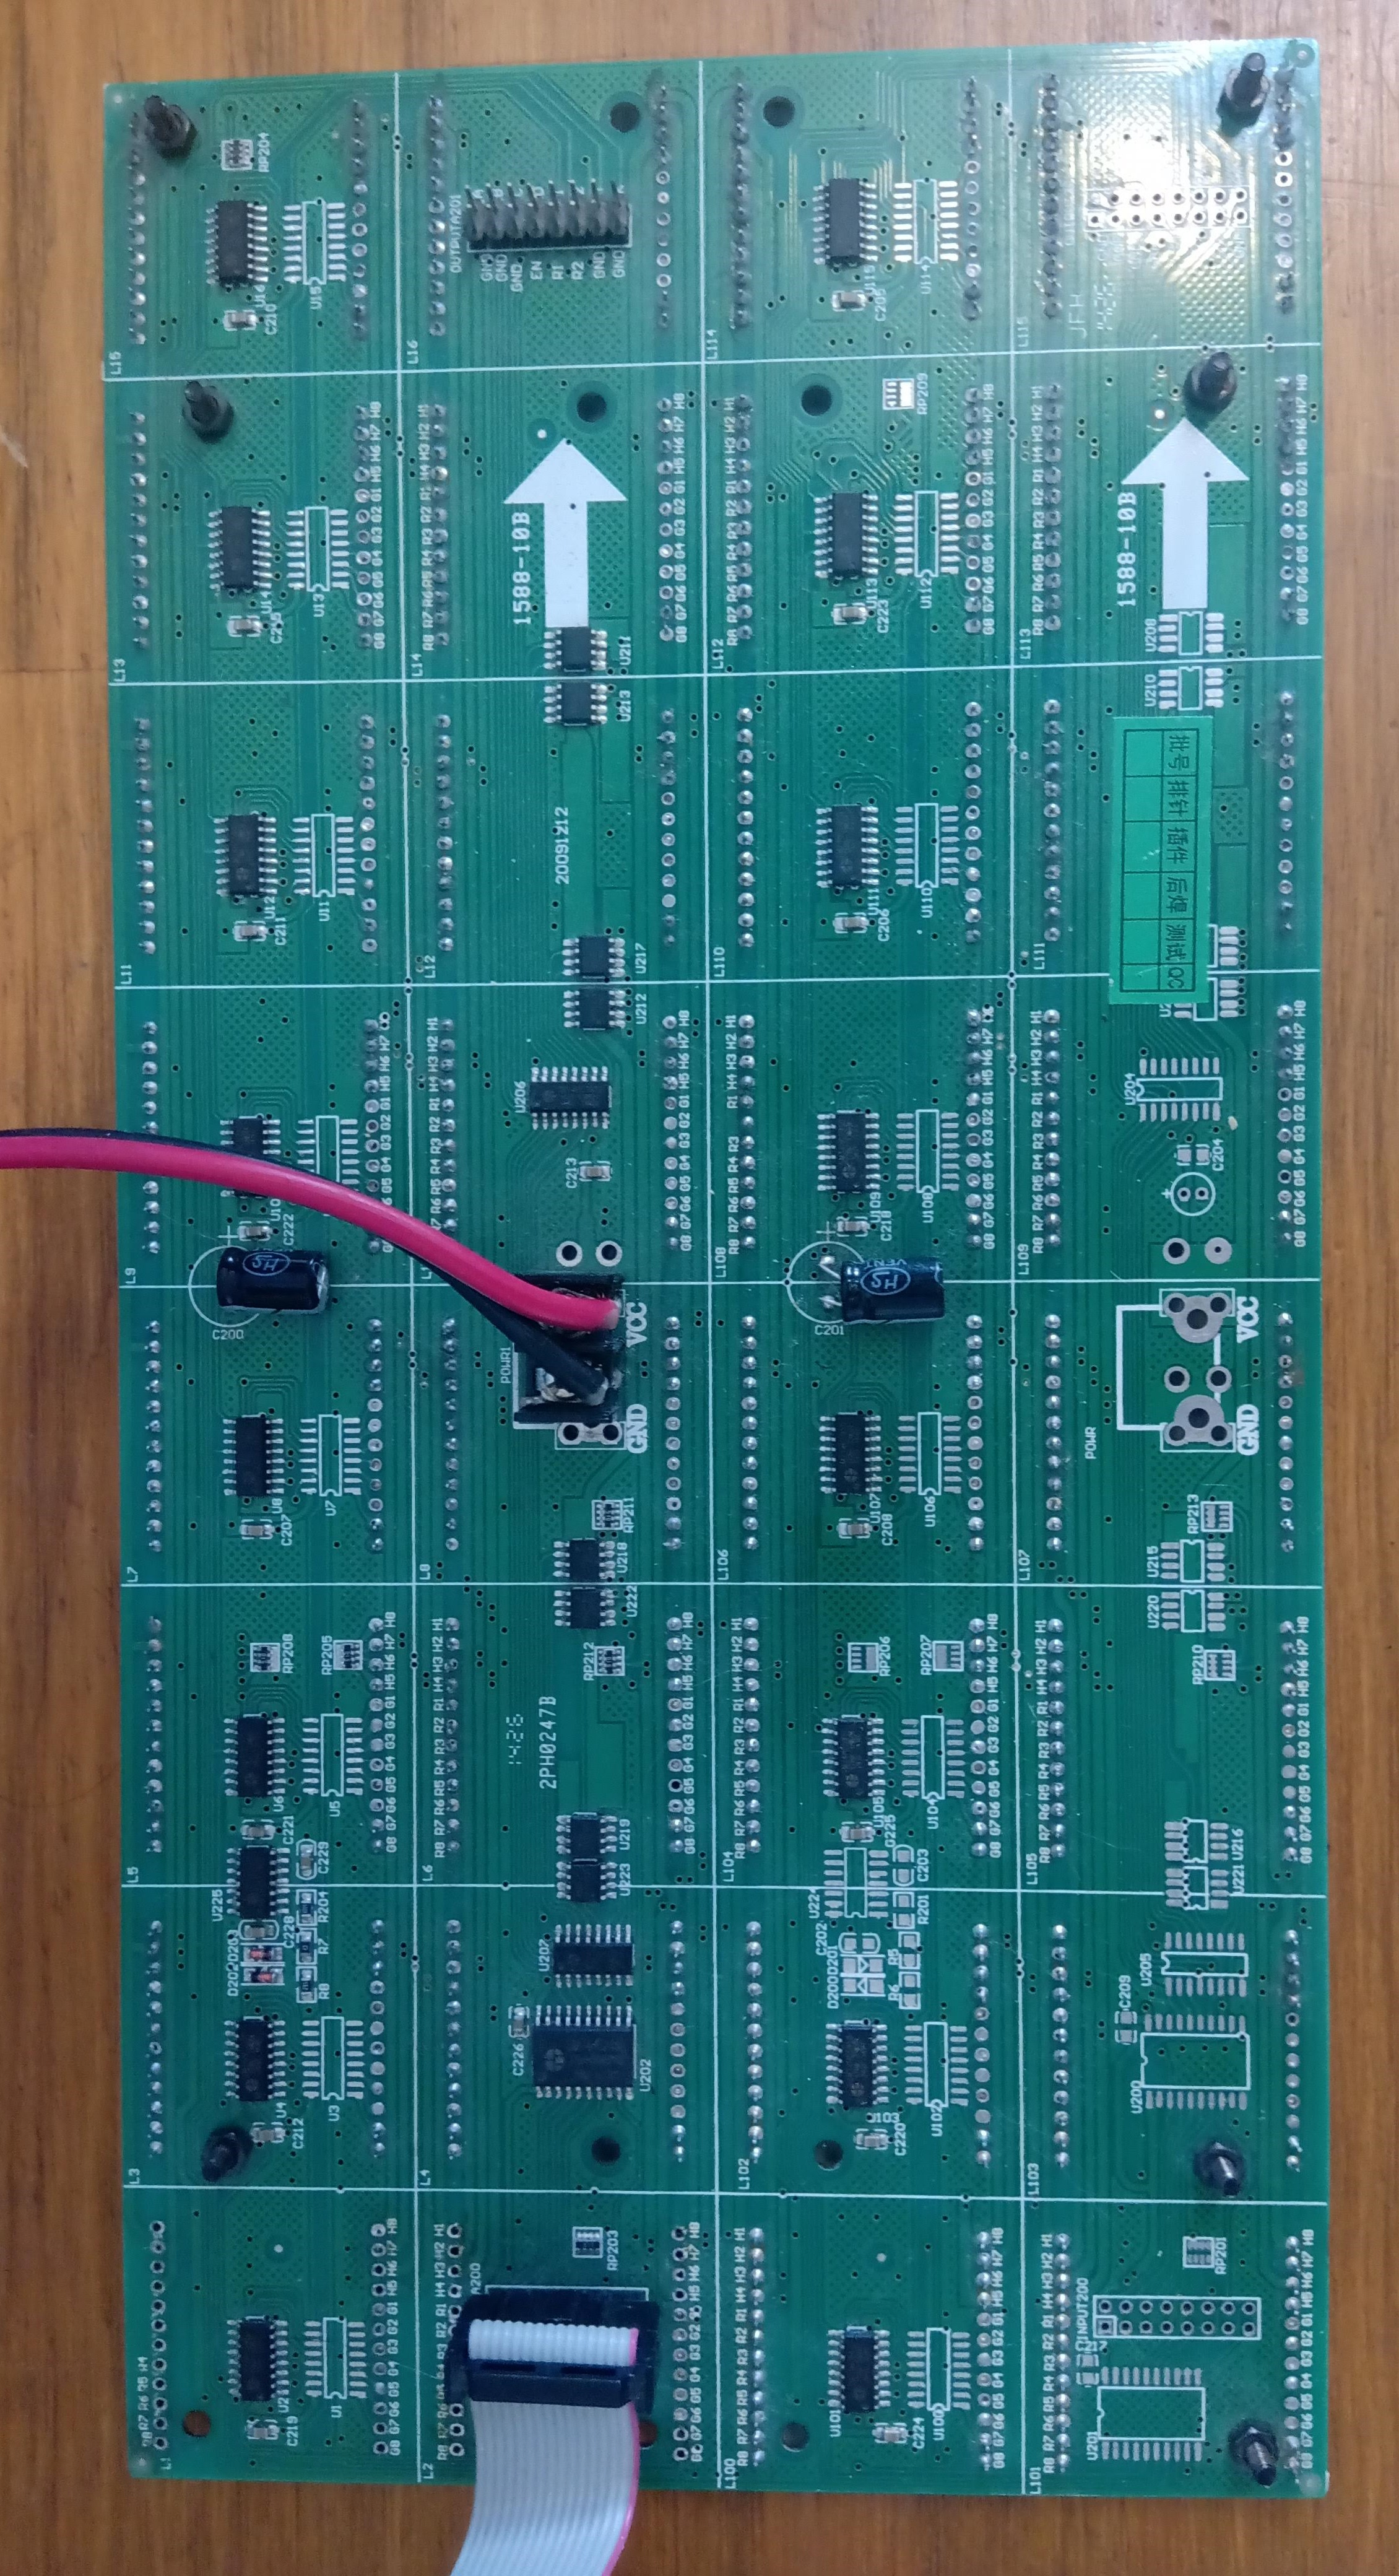
\includegraphics[width=0.75\textwidth, angle=270]{./Figures/cartel4x8.jpg}\\
	\includegraphics[width=1\textwidth]{./Figures/cartelledON.jpg}\\
	\caption{Fotografías de placas de control de los carteles de matriz led: (a) placa de 2x6 módulos; (b) placa de 4x8 módulos; (c) vista posterior de la placa de 4x8.}
	\label{fig:picsDriverled}
\end{figure}


\subsubsection{Placa de control}

\begin{figure}[ht]
	\centering
	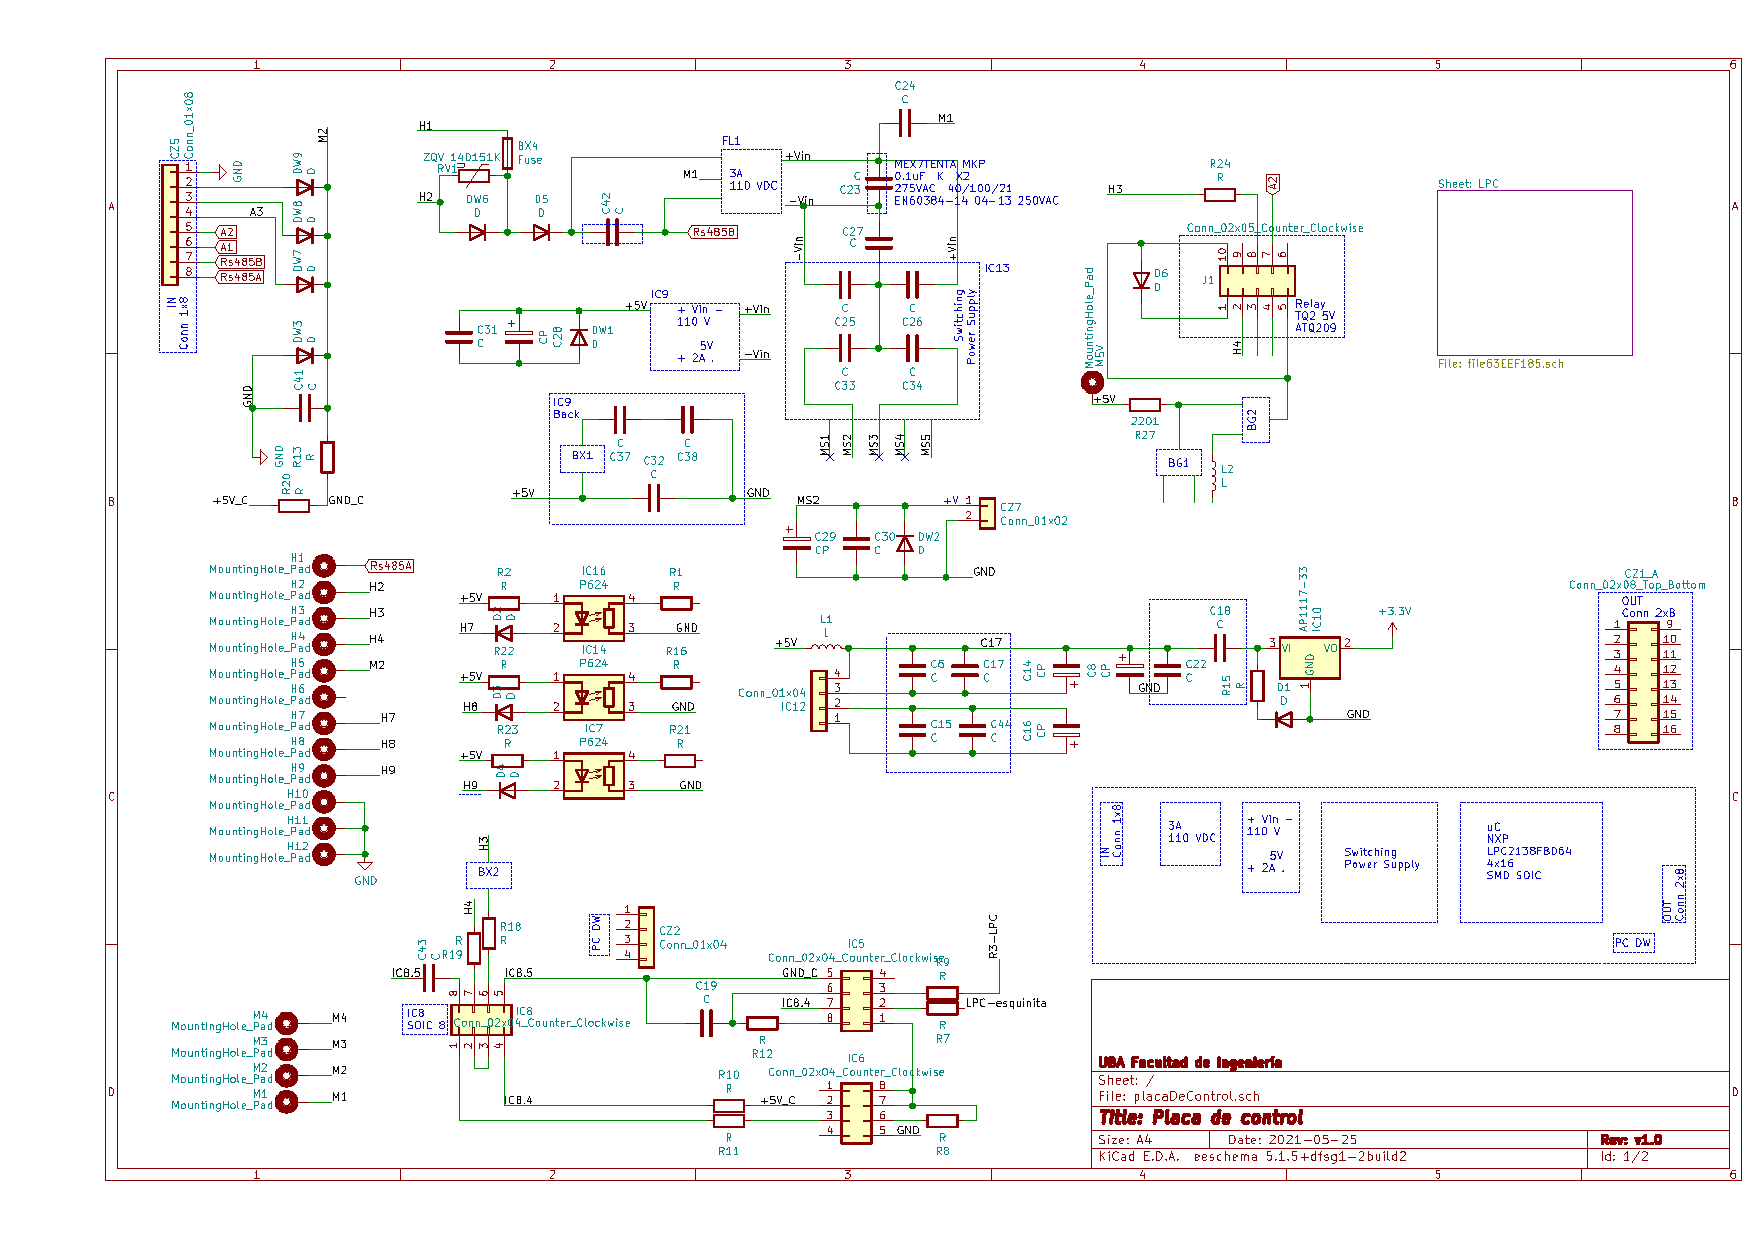
\includegraphics[width=1\textwidth]{./Figures/output.placaControl.pdf}
	\caption{Circuito esquemático de la placa de control de los carteles LED de salón.}
	\label{fig:schController}
\end{figure}


\begin{figure}[ht]
	\centering
	
\includegraphics[width=0.5\textwidth]{./Figures/diagramasTemporales.png}
	\caption{}
	\label{fig:diagramasTemporales}
\end{figure}

\section{Integración con red PIDS}

\section{Pruebas de campo}

\begin{figure}[ht]
	\centering
	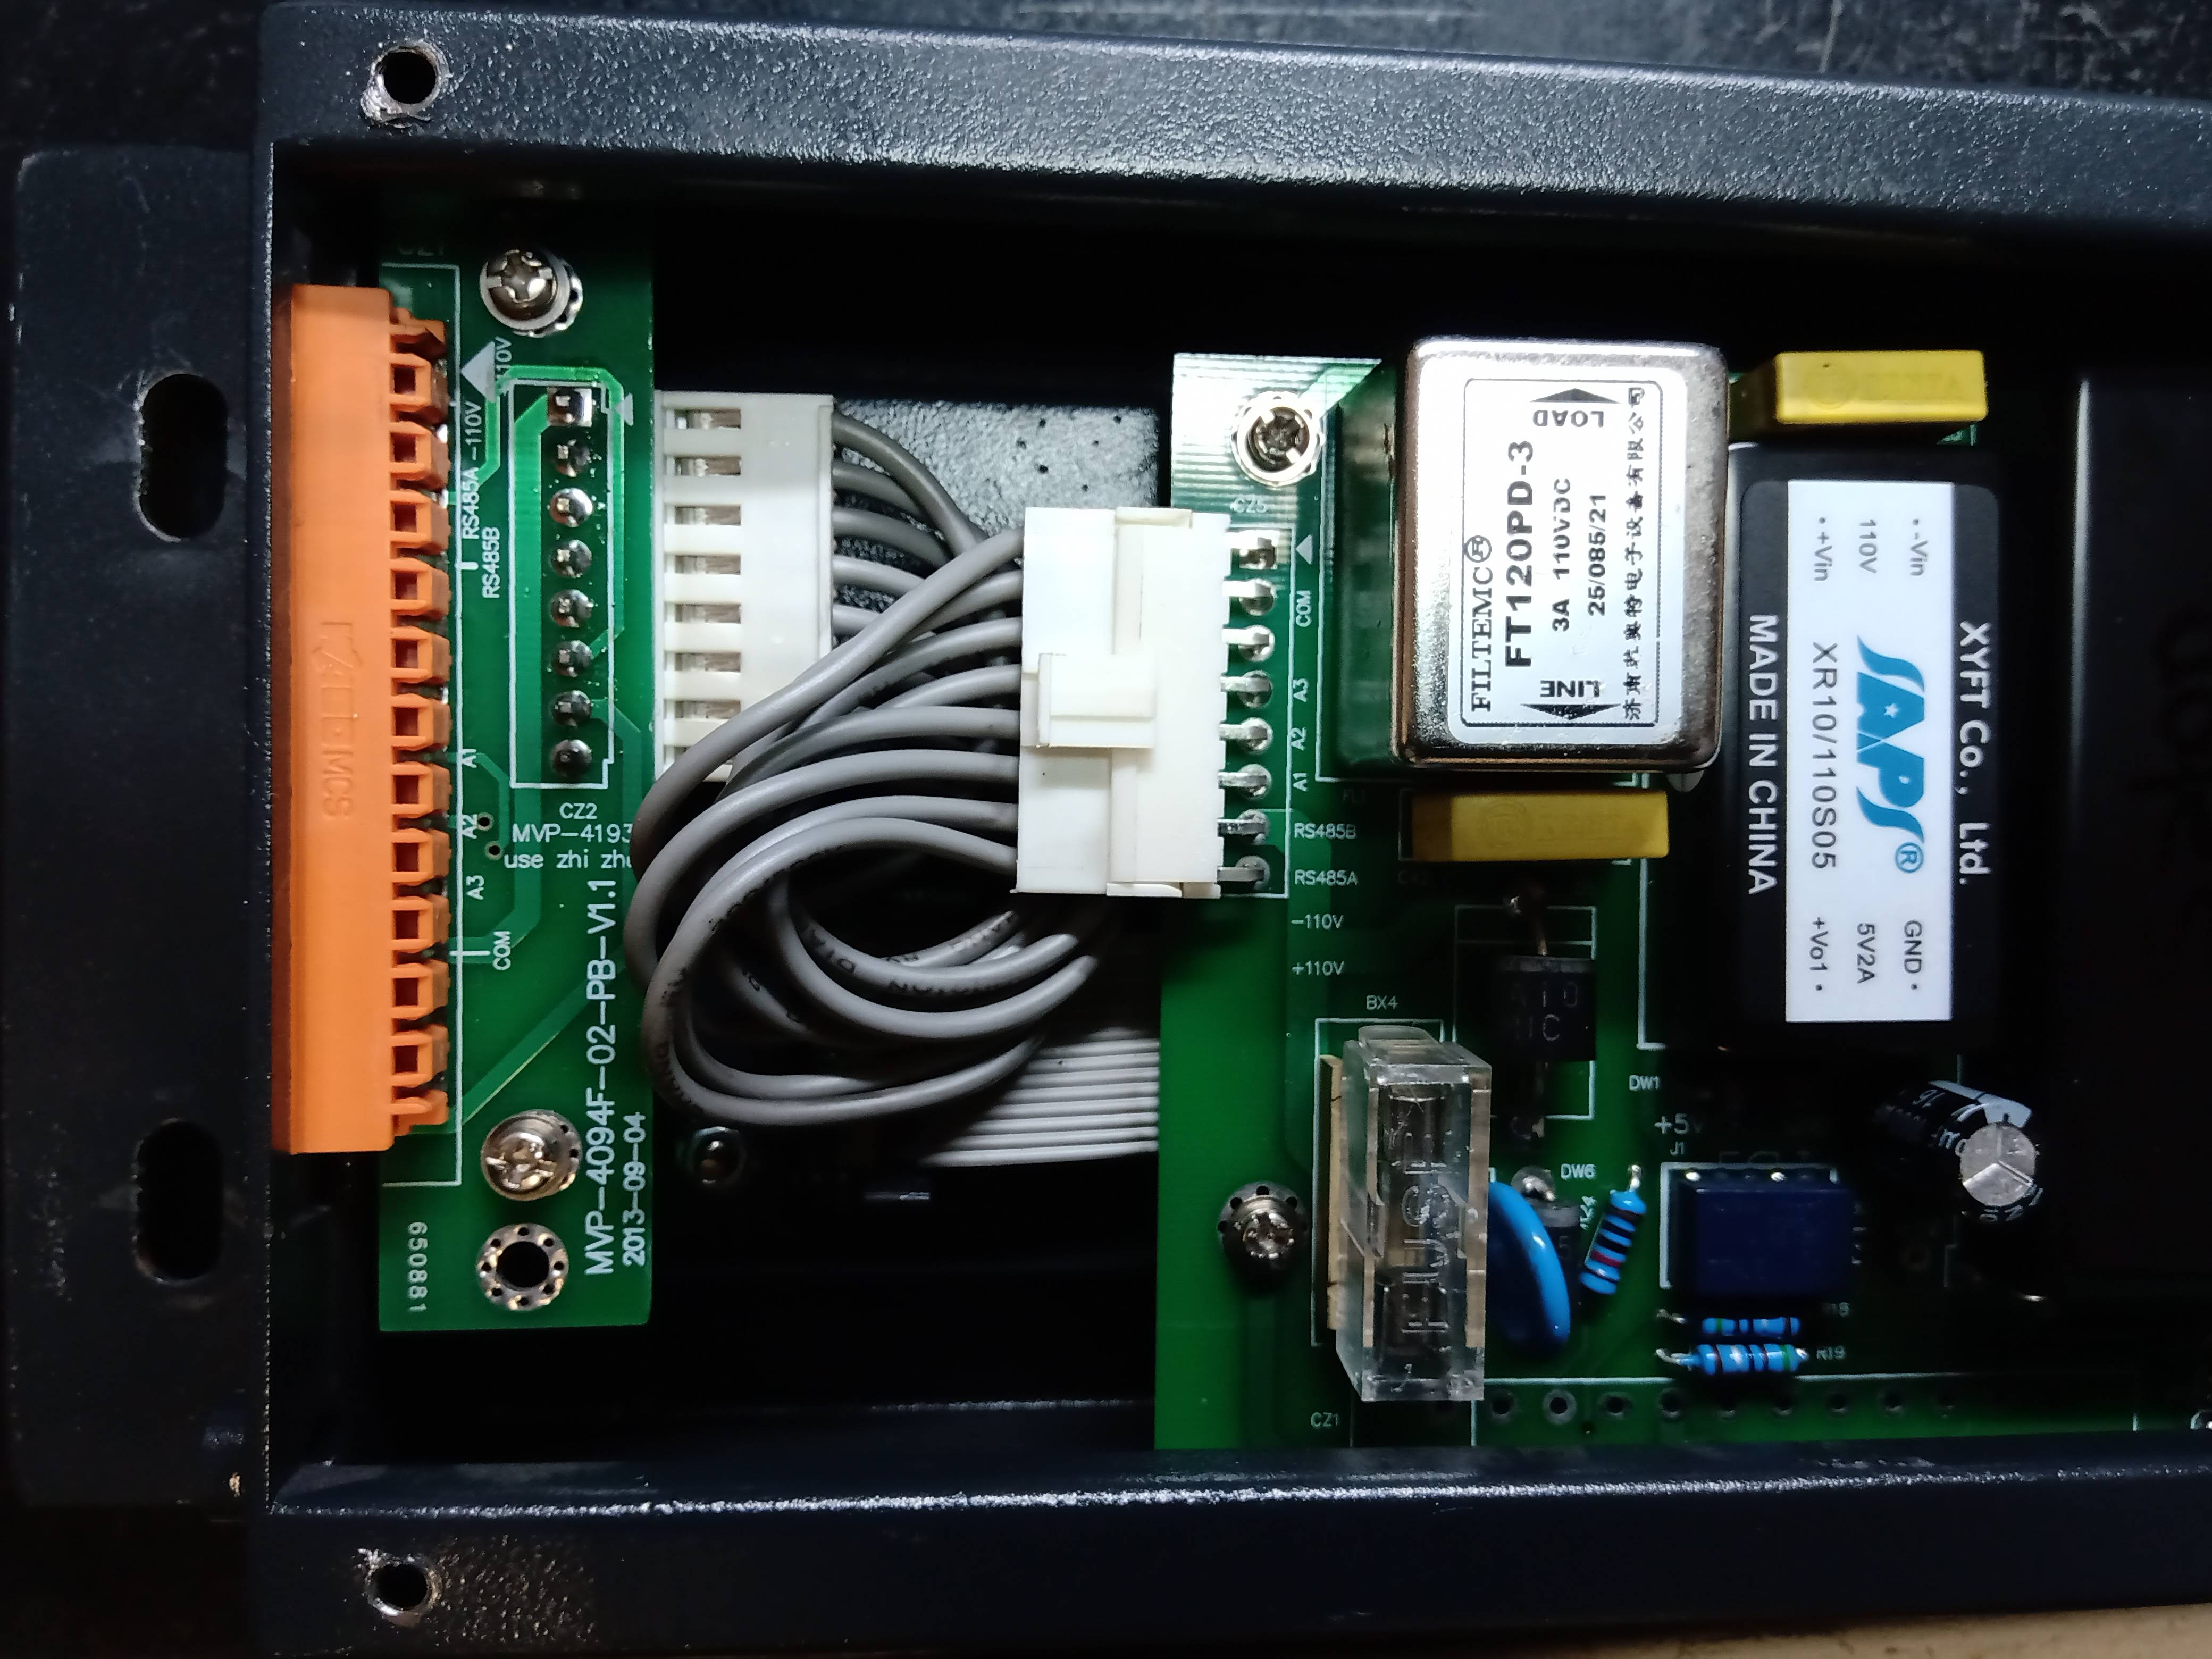
\includegraphics[width=1\textwidth]{./Figures/displayController.jpg}
	\caption{Fotografía del detalle de conexión de la placa de control de los carteles led de salón.}
	\label{fig:displayController}
\end{figure}